\documentclass{article}

\usepackage[utf8]{inputenc}
\usepackage[bottom=2cm, top=2cm, left=2cm, right=2cm]{geometry}
\usepackage{verbatim}
\usepackage{tikz}

\title{Lista - Árvores AVL}
\author{Vinícius Couto Tasso}
\date{}

\begin{document}

\maketitle
\tikzset{every tree node/.style={minimum width=2em,draw,circle},
         blank/.style={draw=none},
         edge from parent/.style=
         {draw,edge from parent path={(\tikzparentnode) -- (\tikzchildnode)}},
         level distance=1cm}
         
\begin{enumerate}

\item Insira as chaves abaixo, na ordem em que são mostradas, em uma árvore AVL inicialmente vazia. Mostre a árvore final (com o fator de balanceamento de cada nó) produzida por essas inserções:

\begin{center}
    \begin{verbatim}
      Q, Z, B, Y, T, M, E, W, X, S, F, G, A, H, N, O, P, R.
    \end{verbatim}
\end{center}

% Insert 5
\begin{center}
    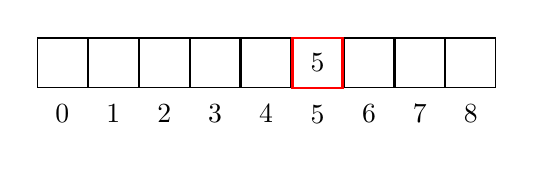
\begin{tikzpicture}
        \tikzstyle{every node}=[draw, minimum size=1.8em]
        
        \matrix[draw=none] {
            \node   (0)    [label=270:$0$] {}; & 
            \node   (1)    [label=270:$1$] {}; &
            \node   (2)    [label=270:$2$] {}; & 
            \node   (3)    [label=270:$3$] {}; &
            \node   (4)    [label=270:$4$] {}; & 
            \node   (5)    [label=270:$5$, draw=red, thick] {5}; &
            \node   (6)    [label=270:$6$] {}; &
            \node   (7)    [label=270:$7$] {}; &
            \node   (8)    [label=270:$8$] {}; \\
        };
        
    \end{tikzpicture}
\end{center}

% Insert 28
\begin{center}
    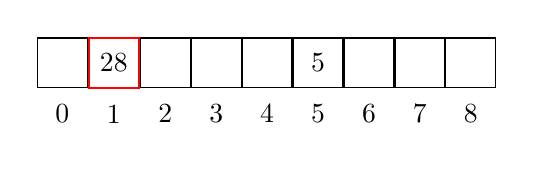
\begin{tikzpicture}
        \tikzstyle{every node}=[draw, minimum size=1.8em]
        
        \matrix[draw=none] {
            \node   (0)    [label=270:$0$] {}; & 
            \node   (1)    [label=270:$1$, draw=red, thick] {28}; &
            \node   (2)    [label=270:$2$] {}; & 
            \node   (3)    [label=270:$3$] {}; &
            \node   (4)    [label=270:$4$] {}; & 
            \node   (5)    [label=270:$5$] {5}; &
            \node   (6)    [label=270:$6$] {}; &
            \node   (7)    [label=270:$7$] {}; &
            \node   (8)    [label=270:$8$] {}; \\
        };
        
    \end{tikzpicture}
\end{center}

% Insert 19
\begin{center}
    \begin{tikzpicture}
        \tikzstyle{every node}=[draw, minimum size=1.8em]
        
        \matrix[draw=none] {
            \node   (0)    [label=270:$0$] {}; & 
            \node   (1)    [label=270:$1$, draw=red, thick] {28}; &
            \node   (2)    [label=270:$2$] {}; & 
            \node   (3)    [label=270:$3$] {}; &
            \node   (4)    [label=270:$4$] {}; & 
            \node   (5)    [label=270:$5$] {5}; &
            \node   (6)    [label=270:$6$] {}; &
            \node   (7)    [label=270:$7$] {}; &
            \node   (8)    [label=270:$8$] {}; \\
        };
        
        \node (1 1) [above=10pt of 1] {19};
        
        \draw[->, color=red] (1) -- (1 1);
        
    \end{tikzpicture}
\end{center}

% Insert 15
\begin{center}
    \begin{tikzpicture}
        \tikzstyle{every node}=[draw, minimum size=1.8em]
        
        \matrix[draw=none] {
            \node   (0)    [label=270:$0$] {}; & 
            \node   (1)    [label=270:$1$] {28}; &
            \node   (2)    [label=270:$2$] {}; & 
            \node   (3)    [label=270:$3$] {}; &
            \node   (4)    [label=270:$4$] {}; & 
            \node   (5)    [label=270:$5$] {5}; &
            \node   (6)    [label=270:$6$, draw=red, thick] {15}; &
            \node   (7)    [label=270:$7$] {}; &
            \node   (8)    [label=270:$8$] {}; \\
        };
        
        \node (1 1) [above=10pt of 1] {19};
        
        \draw[->] (1) -- (1 1);
        
    \end{tikzpicture}
\end{center}

% Insert 20
\begin{center}
    \begin{tikzpicture}
        \tikzstyle{every node}=[draw, minimum size=1.8em]
        
        \matrix[draw=none] {
            \node   (0)    [label=270:$0$] {}; & 
            \node   (1)    [label=270:$1$] {28}; &
            \node   (2)    [label=270:$2$, draw=red, thick] {20}; & 
            \node   (3)    [label=270:$3$] {}; &
            \node   (4)    [label=270:$4$] {}; & 
            \node   (5)    [label=270:$5$] {5}; &
            \node   (6)    [label=270:$6$] {15}; &
            \node   (7)    [label=270:$7$] {}; &
            \node   (8)    [label=270:$8$] {}; \\
        };
        
        \node (1 1) [above=10pt of 1] {19};
        
        \draw[->] (1) -- (1 1);
        
    \end{tikzpicture}
\end{center}

% Insert 33
\begin{center}
    \begin{tikzpicture}
        \tikzstyle{every node}=[draw, minimum size=1.8em]
        
        \matrix[draw=none] {
            \node   (0)    [label=270:$0$] {}; & 
            \node   (1)    [label=270:$1$] {28}; &
            \node   (2)    [label=270:$2$] {20}; & 
            \node   (3)    [label=270:$3$] {}; &
            \node   (4)    [label=270:$4$] {}; & 
            \node   (5)    [label=270:$5$] {5}; &
            \node   (6)    [label=270:$6$, draw=red, thick] {15}; &
            \node   (7)    [label=270:$7$] {}; &
            \node   (8)    [label=270:$8$] {}; \\
        };
        
        \node (1 1) [above=10pt of 1] {19};
        \node (6 1) [above=10pt of 6] {33};
        
        \draw[->] (1) -- (1 1);
        \draw[->, color=red] (6) -- (6 1);
        
    \end{tikzpicture}
\end{center}

% Insert 12
\begin{center}
    \begin{tikzpicture}
        \tikzstyle{every node}=[draw, minimum size=1.8em]
        
        \matrix[draw=none] {
            \node   (0)    [label=270:$0$] {}; & 
            \node   (1)    [label=270:$1$] {28}; &
            \node   (2)    [label=270:$2$] {20}; & 
            \node   (3)    [label=270:$3$, draw=red, thick] {12}; &
            \node   (4)    [label=270:$4$] {}; & 
            \node   (5)    [label=270:$5$] {5}; &
            \node   (6)    [label=270:$6$] {15}; &
            \node   (7)    [label=270:$7$] {}; &
            \node   (8)    [label=270:$8$] {}; \\
        };
        
        \node (1 1) [above=10pt of 1] {19};
        \node (6 1) [above=10pt of 6] {33};
        
        \draw[->] (1) -- (1 1);
        \draw[->] (6) -- (6 1);
        
    \end{tikzpicture}
\end{center}

% Insert 17
\begin{center}
    \begin{tikzpicture}
        \tikzstyle{every node}=[draw, minimum size=1.8em]
        
        \matrix[draw=none] {
            \node   (0)    [label=270:$0$] {}; & 
            \node   (1)    [label=270:$1$] {28}; &
            \node   (2)    [label=270:$2$] {20}; & 
            \node   (3)    [label=270:$3$] {12}; &
            \node   (4)    [label=270:$4$] {}; & 
            \node   (5)    [label=270:$5$] {5}; &
            \node   (6)    [label=270:$6$] {15}; &
            \node   (7)    [label=270:$7$] {}; &
            \node   (8)    [label=270:$8$, draw=red, thick] {17}; \\
        };
        
        \node (1 1) [above=10pt of 1] {19};
        \node (6 1) [above=10pt of 6] {33};
        
        \draw[->] (1) -- (1 1);
        \draw[->] (6) -- (6 1);
        
    \end{tikzpicture}
\end{center}

% Insert 10
\begin{center}
    \begin{tikzpicture}
        \tikzstyle{every node}=[draw, minimum size=1.8em]
        
        \matrix[draw=none] {
            \node   (0)    [label=270:$0$] {}; & 
            \node   (1)    [label=270:$1$, draw=red, thick] {28}; &
            \node   (2)    [label=270:$2$] {20}; & 
            \node   (3)    [label=270:$3$] {12}; &
            \node   (4)    [label=270:$4$] {}; & 
            \node   (5)    [label=270:$5$] {5}; &
            \node   (6)    [label=270:$6$] {15}; &
            \node   (7)    [label=270:$7$] {}; &
            \node   (8)    [label=270:$8$] {17}; \\
        };
        
        \node (1 1) [above=10pt of 1] {19};
        \node (1 2) [above=10pt of 1 1] {10};
        \node (6 1) [above=10pt of 6] {33};
        
        \draw[->, color=red] (1) -- (1 1);
        \draw[->, color=red] (1 1) -- (1 2);
        \draw[->] (6) -- (6 1);
        
    \end{tikzpicture}
\end{center}

\item Mostre cada uma das árvores, assim como o fator de balanceamento de cada nó, após a remoção das chaves a seguir (considere as remoções sobre a árvore final do exercício):

\begin{center}
    \begin{verbatim}
      A, H, E, W, G, N, P, O.
    \end{verbatim}
\end{center}

% Remove A

\begin{center}
    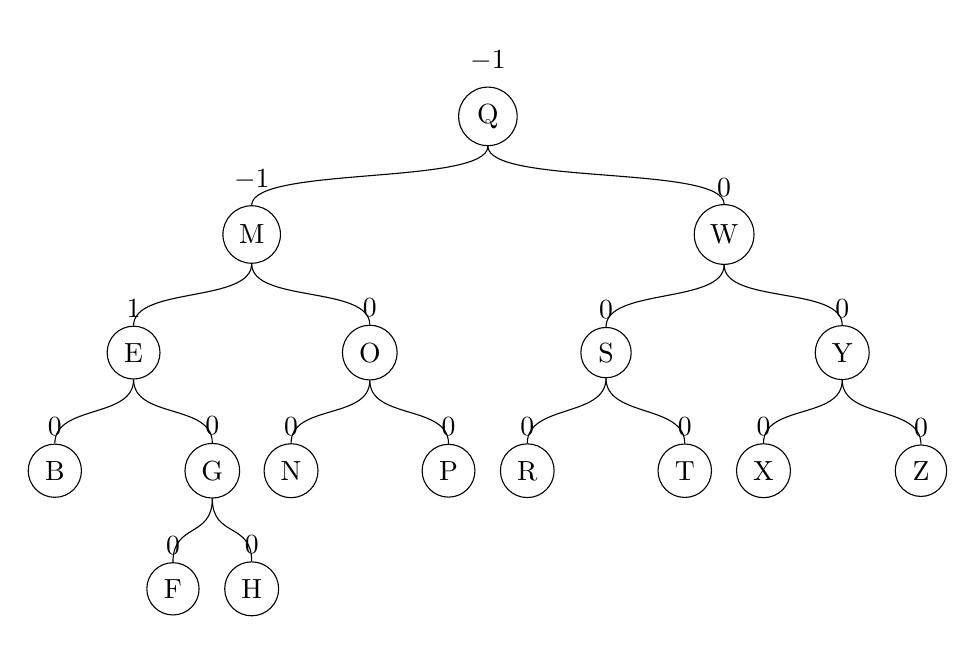
\begin{tikzpicture}[
       edge from parent path=
    {(\tikzparentnode.south) .. controls +(0,-.5) and +(0,.5)
                             .. (\tikzchildnode.north)},
    level 1/.style={sibling distance=6cm},                        
    level 2/.style={sibling distance=3cm},                         
    level 3/.style={sibling distance=2cm},
    level 4/.style={sibling distance=1cm},
   every node/.style={draw,circle},
   label distance=-1mm]
   
\node[label=90:$-1$] {Q}
    child {node[label=90:$-1$] {M}
        child {node[label=90:$1$] {E}
            child {node[label=90:$0$] {B}}
            child {node[label=90:$0$] {G}
                child {node[label=90:$0$] {F}}
                child {node[label=90:$0$] {H}}
            }
        }
        child {node[label=90:$0$] {O}
            child {node[label=90:$0$] {N}}
            child {node[label=90:$0$] {P}}
        }
    }   
    child {node[label=90:$0$] {W}
        child {node[label=90:$0$] {S}
            child {node[label=90:$0$] {R}}
            child {node[label=90:$0$] {T}}
            }
        child {node[label=90:$0$] {Y}
            child {node[label=90:$0$] {X}}
            child {node[label=90:$0$] {Z}}
            }
    };

\end{tikzpicture}
\end{center}

% Remove H

\begin{center}
    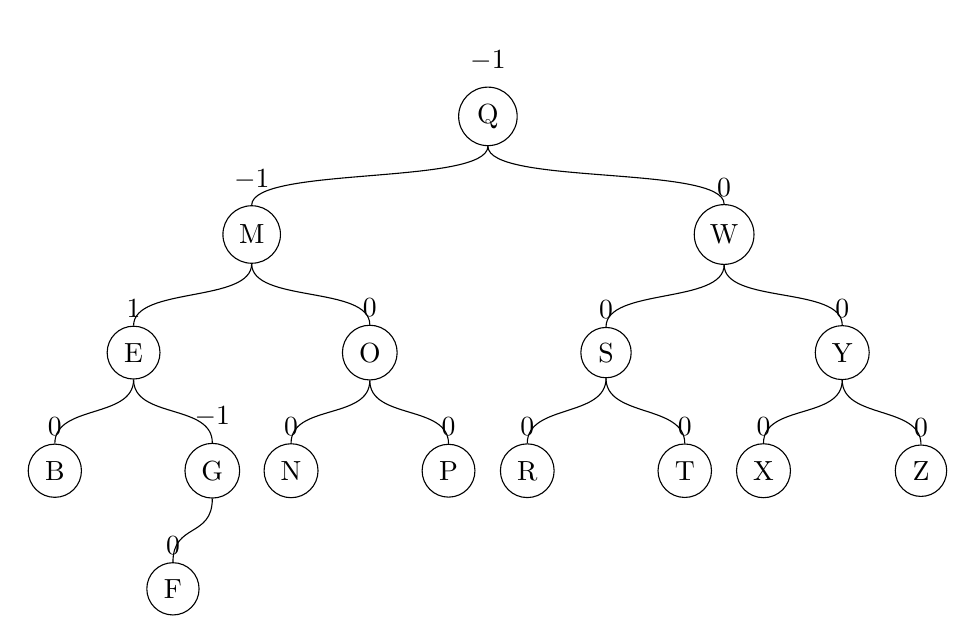
\begin{tikzpicture}[
       edge from parent path=
    {(\tikzparentnode.south) .. controls +(0,-.5) and +(0,.5)
                             .. (\tikzchildnode.north)},
    level 1/.style={sibling distance=6cm},                        
    level 2/.style={sibling distance=3cm},                         
    level 3/.style={sibling distance=2cm},
    level 4/.style={sibling distance=1cm},
   every node/.style={draw,circle},
   label distance=-1mm]
   
\node[label=90:$-1$] {Q}
    child {node[label=90:$-1$] {M}
        child {node[label=90:$1$] {E}
            child {node[label=90:$0$] {B}}
            child {node[label=90:$-1$] {G}
                child {node[label=90:$0$] {F}}
                child[missing]{}
            }
        }
        child {node[label=90:$0$] {O}
            child {node[label=90:$0$] {N}}
            child {node[label=90:$0$] {P}}
        }
    }   
    child {node[label=90:$0$] {W}
        child {node[label=90:$0$] {S}
            child {node[label=90:$0$] {R}}
            child {node[label=90:$0$] {T}}
            }
        child {node[label=90:$0$] {Y}
            child {node[label=90:$0$] {X}}
            child {node[label=90:$0$] {Z}}
            }
    };

\end{tikzpicture}
\end{center}

% Remove E

\begin{center}
    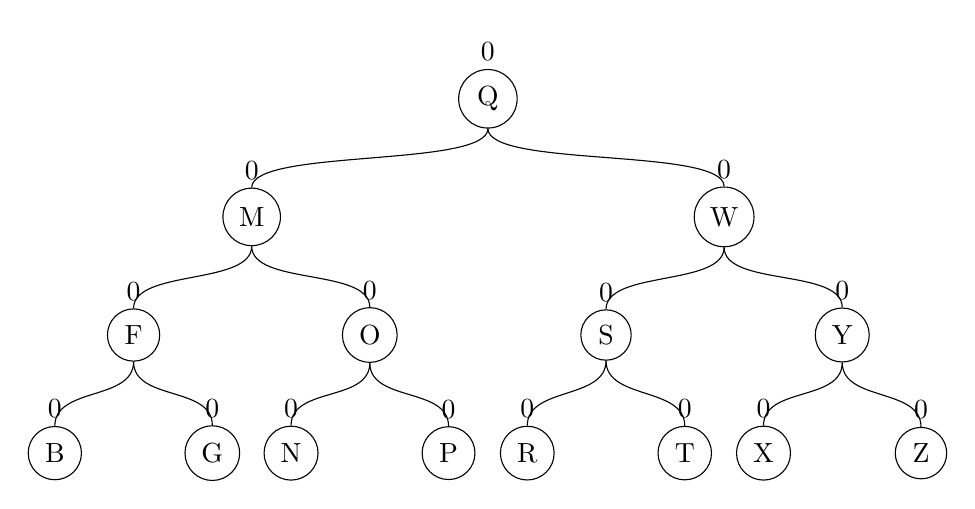
\begin{tikzpicture}[
       edge from parent path=
    {(\tikzparentnode.south) .. controls +(0,-.5) and +(0,.5)
                             .. (\tikzchildnode.north)},
    level 1/.style={sibling distance=6cm},                        
    level 2/.style={sibling distance=3cm},                         
    level 3/.style={sibling distance=2cm},
   every node/.style={draw,circle},
   label distance=-1mm]
   
\node[label=90:$0$] {Q}
    child {node[label=90:$0$] {M}
        child {node[label=90:$0$] {F}
            child {node[label=90:$0$] {B}}
            child {node[label=90:$0$] {G}}
        }
        child {node[label=90:$0$] {O}
            child {node[label=90:$0$] {N}}
            child {node[label=90:$0$] {P}}
        }
    }   
    child {node[label=90:$0$] {W}
        child {node[label=90:$0$] {S}
            child {node[label=90:$0$] {R}}
            child {node[label=90:$0$] {T}}
            }
        child {node[label=90:$0$] {Y}
            child {node[label=90:$0$] {X}}
            child {node[label=90:$0$] {Z}}
            }
    };

\end{tikzpicture}
\end{center}

% Remove W

\begin{center}
    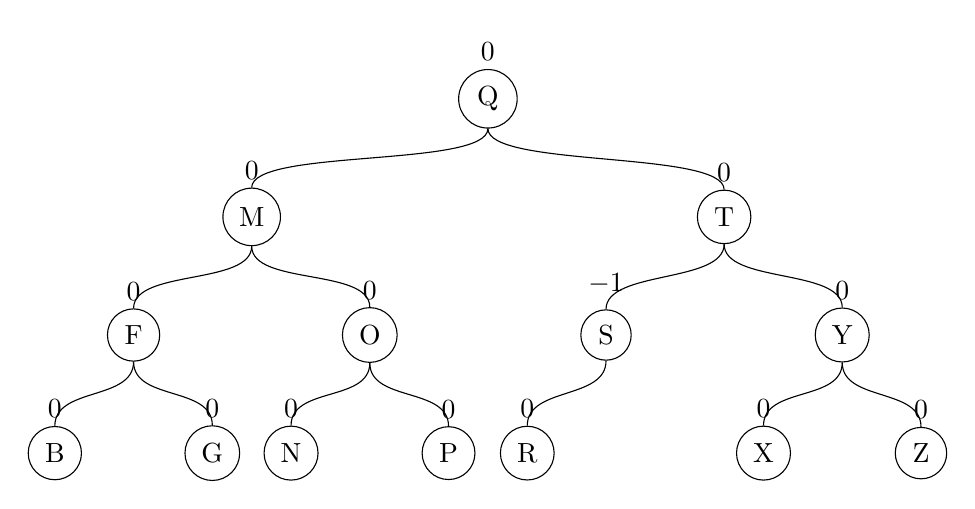
\begin{tikzpicture}[
       edge from parent path=
    {(\tikzparentnode.south) .. controls +(0,-.5) and +(0,.5)
                             .. (\tikzchildnode.north)},
    level 1/.style={sibling distance=6cm},                        
    level 2/.style={sibling distance=3cm},                         
    level 3/.style={sibling distance=2cm},
   every node/.style={draw,circle},
   label distance=-1mm]
   
\node[label=90:$0$] {Q}
    child {node[label=90:$0$] {M}
        child {node[label=90:$0$] {F}
            child {node[label=90:$0$] {B}}
            child {node[label=90:$0$] {G}}
        }
        child {node[label=90:$0$] {O}
            child {node[label=90:$0$] {N}}
            child {node[label=90:$0$] {P}}
        }
    }   
    child {node[label=90:$0$] {T}
        child {node[label=90:$-1$] {S}
            child {node[label=90:$0$] {R}}
            child[missing]{}
            }
        child {node[label=90:$0$] {Y}
            child {node[label=90:$0$] {X}}
            child {node[label=90:$0$] {Z}}
            }
    };

\end{tikzpicture}
\end{center}

% Remove G

\begin{center}
    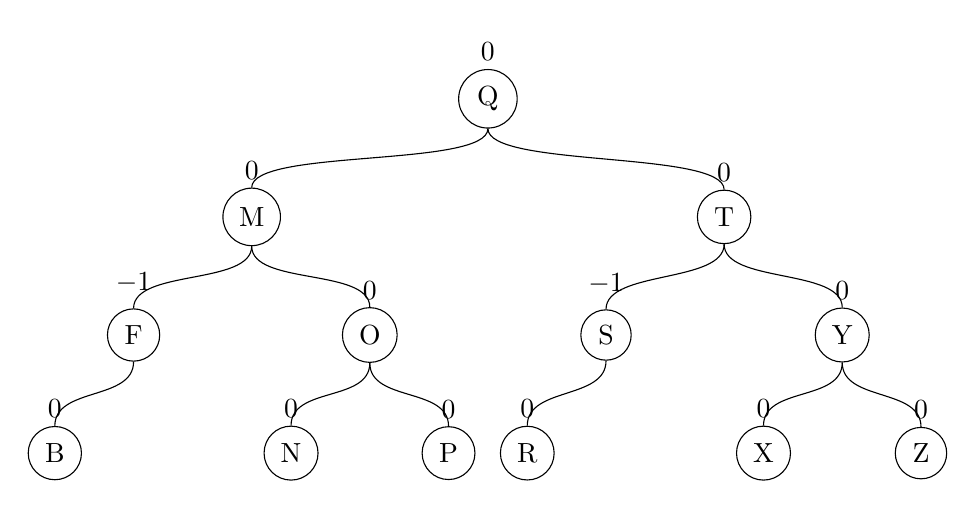
\begin{tikzpicture}[
       edge from parent path=
    {(\tikzparentnode.south) .. controls +(0,-.5) and +(0,.5)
                             .. (\tikzchildnode.north)},
    level 1/.style={sibling distance=6cm},                        
    level 2/.style={sibling distance=3cm},                         
    level 3/.style={sibling distance=2cm},
   every node/.style={draw,circle},
   label distance=-1mm]
   
\node[label=90:$0$] {Q}
    child {node[label=90:$0$] {M}
        child {node[label=90:$-1$] {F}
            child {node[label=90:$0$] {B}}
            child[missing]{}
        }
        child {node[label=90:$0$] {O}
            child {node[label=90:$0$] {N}}
            child {node[label=90:$0$] {P}}
        }
    }   
    child {node[label=90:$0$] {T}
        child {node[label=90:$-1$] {S}
            child {node[label=90:$0$] {R}}
            child[missing]{}
            }
        child {node[label=90:$0$] {Y}
            child {node[label=90:$0$] {X}}
            child {node[label=90:$0$] {Z}}
            }
    };

\end{tikzpicture}
\end{center}

% Remove N

\begin{center}
    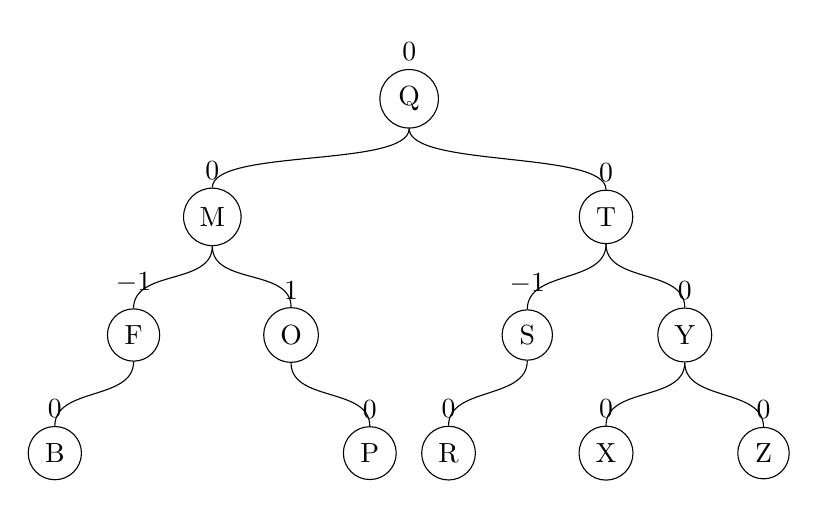
\begin{tikzpicture}[
       edge from parent path=
    {(\tikzparentnode.south) .. controls +(0,-.5) and +(0,.5)
                             .. (\tikzchildnode.north)},
    level 1/.style={sibling distance=5cm},                        
    level 2/.style={sibling distance=2cm},                         
    level 3/.style={sibling distance=2cm},
   every node/.style={draw,circle},
   label distance=-1mm]
   
\node[label=90:$0$] {Q}
    child {node[label=90:$0$] {M}
        child {node[label=90:$-1$] {F}
            child {node[label=90:$0$] {B}}
            child[missing]{}
        }
        child {node[label=90:$1$] {O}
            child[missing]{}
            child {node[label=90:$0$] {P}}
        }
    }   
    child {node[label=90:$0$] {T}
        child {node[label=90:$-1$] {S}
            child {node[label=90:$0$] {R}}
            child[missing]{}
            }
        child {node[label=90:$0$] {Y}
            child {node[label=90:$0$] {X}}
            child {node[label=90:$0$] {Z}}
            }
    };

\end{tikzpicture}
\end{center}

% Remove P

\begin{center}
    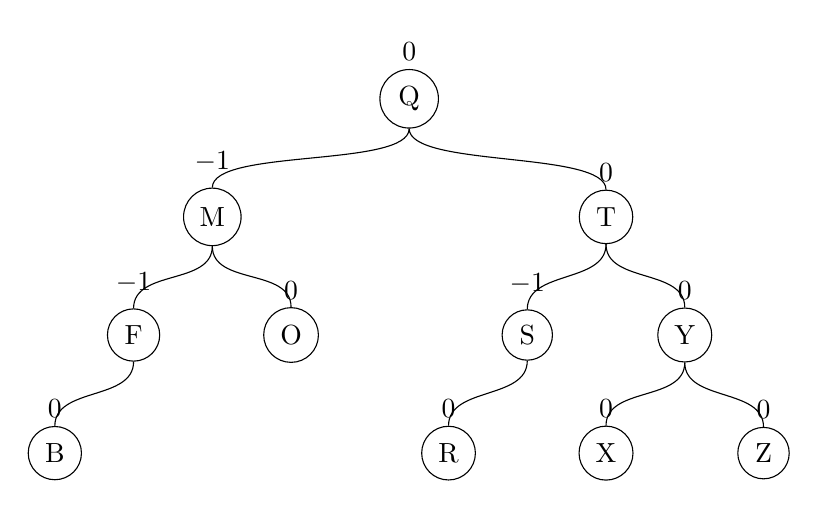
\begin{tikzpicture}[
       edge from parent path=
    {(\tikzparentnode.south) .. controls +(0,-.5) and +(0,.5)
                             .. (\tikzchildnode.north)},
    level 1/.style={sibling distance=5cm},                        
    level 2/.style={sibling distance=2cm},                         
    level 3/.style={sibling distance=2cm},
   every node/.style={draw,circle},
   label distance=-1mm]
   
\node[label=90:$0$] {Q}
    child {node[label=90:$-1$] {M}
        child {node[label=90:$-1$] {F}
            child {node[label=90:$0$] {B}}
            child[missing]{}
        }
        child {node[label=90:$0$] {O}}
    }   
    child {node[label=90:$0$] {T}
        child {node[label=90:$-1$] {S}
            child {node[label=90:$0$] {R}}
            child[missing]{}
            }
        child {node[label=90:$0$] {Y}
            child {node[label=90:$0$] {X}}
            child {node[label=90:$0$] {Z}}
            }
    };

\end{tikzpicture}
\end{center}

% Remove O

\begin{center}
    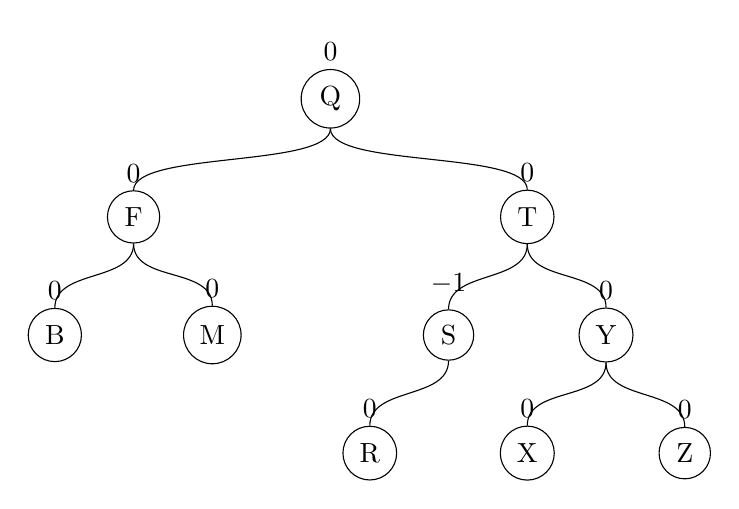
\begin{tikzpicture}[
       edge from parent path=
    {(\tikzparentnode.south) .. controls +(0,-.5) and +(0,.5)
                             .. (\tikzchildnode.north)},
    level 1/.style={sibling distance=5cm},                        
    level 2/.style={sibling distance=2cm},                         
    level 3/.style={sibling distance=2cm},
   every node/.style={draw,circle},
   label distance=-1mm]
   
\node[label=90:$0$] {Q}
    child {node[label=90:$0$] {F}
        child {node[label=90:$0$] {B}}
        child {node[label=90:$0$] {M}}
    }   
    child {node[label=90:$0$] {T}
        child {node[label=90:$-1$] {S}
            child {node[label=90:$0$] {R}}
            child[missing]{}
            }
        child {node[label=90:$0$] {Y}
            child {node[label=90:$0$] {X}}
            child {node[label=90:$0$] {Z}}
            }
    };

\end{tikzpicture}
\end{center}

\item Mostre a árvore final após a remoção do nó com chave 1.


\begin{center}
    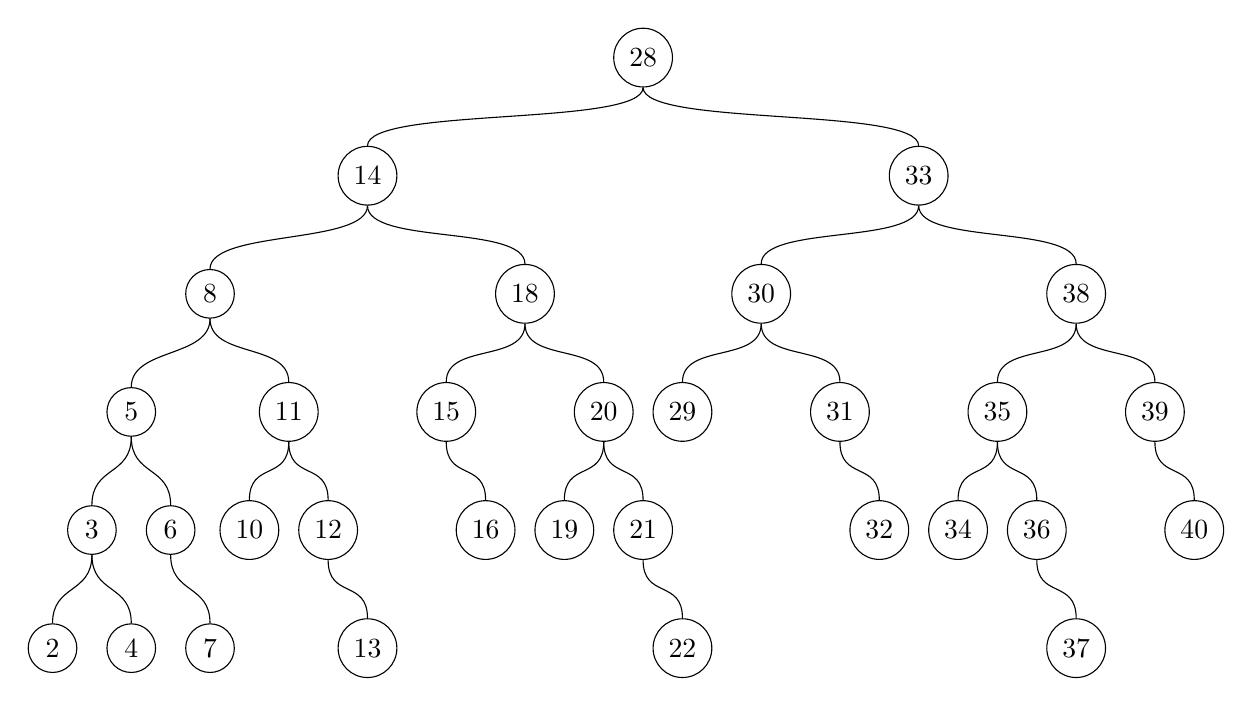
\begin{tikzpicture}[
       edge from parent path=
    {(\tikzparentnode.south) .. controls +(0,-.5) and +(0,.5)
                             .. (\tikzchildnode.north)},
    level 1/.style={sibling distance=7cm},                        
    level 2/.style={sibling distance=4cm},                         
    level 3/.style={sibling distance=2cm},
    level 4/.style={sibling distance=1cm},
   every node/.style={draw,circle},
   label distance=-1mm]
   
\node {28}
    child {node {14}
        child {node {8}
            child {node {5}
                child {node {3}
                    child {node {2}}
                    child {node {4}}
                }
                child {node {6}
                    child[missing] {}
                    child {node {7}}
                }
            }
            child {node {11}
                child {node {10}}
                child {node {12}
                    child[missing] {}   
                    child {node {13}}
                }
            }
        }
        child {node {18}
            child {node {15}
                child[missing] {}   
                child {node {16}}
            }
            child {node {20}
                child {node {19}}
                child {node {21}
                    child[missing] {}   
                    child {node {22}}
                }
            }
        }
    }   
    child {node {33}
        child {node {30}
            child {node {29}}
            child {node {31}
                    child[missing] {}
                    child {node {32}}
                }
            }
        child {node {38}
            child {node {35}
                child {node {34}}
                child {node {36}
                    child[missing] {}
                    child {node {37}}
                }
            }
            child {node {39}
                child[missing] {}
                child {node {40}}
            }
        }
    };

\end{tikzpicture}
\end{center}

\end{enumerate}

\end{document}
